\documentclass{beamer}

\usepackage[ngerman]{babel}
\usepackage[utf8]{inputenc}
\usepackage{hyperref}
\usepackage{pdfpages}

\mode<presentation>{
	\definecolor{LogoRed}{RGB}{219,00,31}
	\definecolor{LogoGray}{RGB}{86,86,80}

	\useoutertheme[width=2.1cm]{sidebar}
	\useinnertheme{rounded}
	\setbeamercolor{normal text}{fg=black,bg=white}
	\setbeamercolor{palette sidebar primary}{use=normal text,fg=normal text.fg}
	\setbeamercolor{title}{fg=LogoRed}
	\setbeamercolor{frametitle}{fg=LogoRed}
	\setbeamercolor{structure}{fg=LogoRed}
	\setbeamercolor{section in sidebar}{fg=LogoRed}
	\setbeamercolor{subsection in sidebar}{fg=LogoRed}

	\usefoottemplate{\vbox{\tinycolouredline{LogoGray!25}{\hspace{4pt}\hspace{15pt}\insertdate\hfill\insertshortinstitute\hfill \insertframenumber{}/\inserttotalframenumber}}}

	\setbeamertemplate{section in toc}{\inserttocsectionnumber.~\inserttocsection\par}
	\setbeamertemplate{subsection in toc}{\hspace*{2em}\inserttocsectionnumber.\inserttocsubsectionnumber~\inserttocsubsection}
	\AtBeginSubsection[] {
		\begin{frame}<beamer>
		\frametitle{Outline}
		\tableofcontents[currentsection,sectionstyle=show/show,subsectionstyle=show/shaded/hide]
		\end{frame}
	}
}

\begin{document}

\title{Einführung Vorkurs WS 2014/2015}
\author[Thomas Maier]{Thomas Maier\\\texttt{tmaier@fs.cs.hm.edu}}
\institute[Fachschaft 07]{Fachschaft 07\\Hochschule München}
\logo{
\includegraphics[height=1.5cm]{logo_fs07.pdf}}

\setbeamertemplate{navigation symbols}{}

\frame{\titlepage}



\section*{Begrüßung}
\begin{frame}
\frametitle{Vorstellung}
\begin{itemize}
	\item Orga
		\begin{itemize}
			\item Thomas Maier
			\item Diana Irmscher
		\end{itemize}
	\item Dozenten
\end{itemize}
\end{frame}

\begin{frame}
\frametitle{Inhalt}
\tableofcontents
\end{frame}


\section{Termine}
\begin{frame}
\frametitle{Termine}
\begin{itemize}
	\item Ersti-Tag\\Roter Würfel (R1.046)\\1. Oktober um 14:00
	\pause
	\item SVV\\R0.058\\Dezember
	\pause
	\item Wahl der AW-Fächer
	\pause
		\begin{itemize}
			\item 18.09. bis 03.10. $\Rightarrow$ 1. Losdurchgang
			\item 06.09. bis 07.10. $\Rightarrow$ 2. Losdurchgang
			\item Danach $\Rightarrow$ Persönliche Nachbelegung
		\end{itemize}
\end{itemize}
\end{frame}


\section{Die Fachschaft}
\begin{frame}
\frametitle{Die Fachschaft}

\begin{center}
\pause

\includegraphics[width=1.9cm]{img/benni1.jpg}
\pause
\hspace{0.1cm}

\includegraphics[width=1.9cm]{img/benni2.jpg}
\pause
\hspace{0.1cm}

\includegraphics[width=1.9cm]{img/benni3.jpg}\\
\pause
\vspace{0.2cm}

\includegraphics[width=1.9cm]{img/benni4.jpg}
\pause
\hspace{0.1cm}

\includegraphics[width=1.9cm]{img/benni5.jpg}
\pause
\hspace{0.1cm}

\includegraphics[width=1.9cm]{img/benni6.jpg}
\vspace{0.1cm}


\end{center}
\end{frame}


\section{Das Studium}
\begin{frame}
\frametitle{Accounts}

\begin{itemize}
	\item Hochschul-Account: \texttt{yourname@hm.edu}
		\begin{itemize}
			\item Mail-Postfach\\
				\footnotesize\url{https://portal.hm.edu/webmail/}\small
			\pause
			\item Moodle (E-Learning-Plattform)\\
				\footnotesize\url{https://moodle.hm.edu/}\small
			\pause
			\item Eduroam (WLAN)\\
				\footnotesize\url{http://www.lrz.de/services/netz/mobil/wireless/}\small
			\pause
			\item LRZ (VPN/WLAN)\\
				\footnotesize\url{https://www.lrz.de/services/netz/mobil/vpn/}\small
		\end{itemize}
	\pause
	\item IFW-Account: \texttt{ifw13370}
		\begin{itemize}
			\item Laborrechner
			\pause
			\item ZPA\\
				\footnotesize\url{https://w3-o.cs.hm.edu/zpa/}\small
		\end{itemize}
\end{itemize}
\end{frame}


\begin{frame}
\frametitle{Veranstaltungen}
\begin{itemize}
	\item Anwesenheitspflicht in Vorlesungen?
		\begin{itemize}
			\item Meistens nein, wenn doch sagt euch das der Prof
			\item Trotzdem ratsam alle zu besuchen!
		\end{itemize}
	\pause
	\item Zwischen Vorlesungen
		\begin{itemize}
			\item Lernen, Essen, Entspannen
			\item Aufenthaltsräume
		\end{itemize}
	\pause
	\item Nach Vorlesungen
		\begin{itemize}
			\item Lernen
			\item Abgaben
		\end{itemize}
\end{itemize}
\end{frame}


\begin{frame}
\frametitle{Tipps (1)}
\begin{itemize}
	\item Lerngruppen: Anzahl wichtig
	\pause
	\item Wahl des Praktikumspartners
	\pause
	\item Prüfungen schieben: Nach Möglichkeit garnicht! Dadurch verlängert sich fast zwangsläufig das Studium!
	\pause
	\item Eigenes Notebook: Empfehlenswert
	\pause
	\item Bücher kaufen: Meist unnötig, genug ausleihbar\\
		\footnotesize Bib: \url{http://www.bib.hm.edu/}\small
\end{itemize}
\end{frame}


\begin{frame}
\frametitle{Tipps (2)}
\begin{itemize}
	\item Unterlagen, Skripte
		\begin{itemize}
			\item Moodle, Mitschriften, Skriptensammlung
			\item Skriptenbestellung in der Fachschaft
		\end{itemize}
	\pause
	\item Website der Fachschaft: \scriptsize\url{http://fs.cs.hm.edu/}\normalsize
		\begin{itemize}
			\item Infos, Hilfestellungen
			\item Sortiertes Schwarzes Brett
			\item Raumsuche
			\item Prof-Suche
			\item Stellenanzeigen
		\end{itemize}
	\pause
	\item Android-App der Fachschaft\\
		\scriptsize\url{https://play.google.com/store/apps/details?id=com.fk07}\normalsize
\end{itemize}
\end{frame}


\section{Vorkurs}
\begin{frame}
\frametitle{Vorkurs}
\begin{itemize}
	\item Softwareentwicklung
		\begin{itemize}
			\item Nötige Grundlagen
			\item Einführung ins Programmieren mit Java
		\end{itemize}
	\pause
	\item Mathematik
		\begin{itemize}
			\item Vorlesungen
			\item Übungen
		\end{itemize}
\end{itemize}
\end{frame}


\begin{frame}
\frametitle{Gruppeneinteilung}
\end{frame}

{
	\setbeamercolor{background canvas}{bg=}
	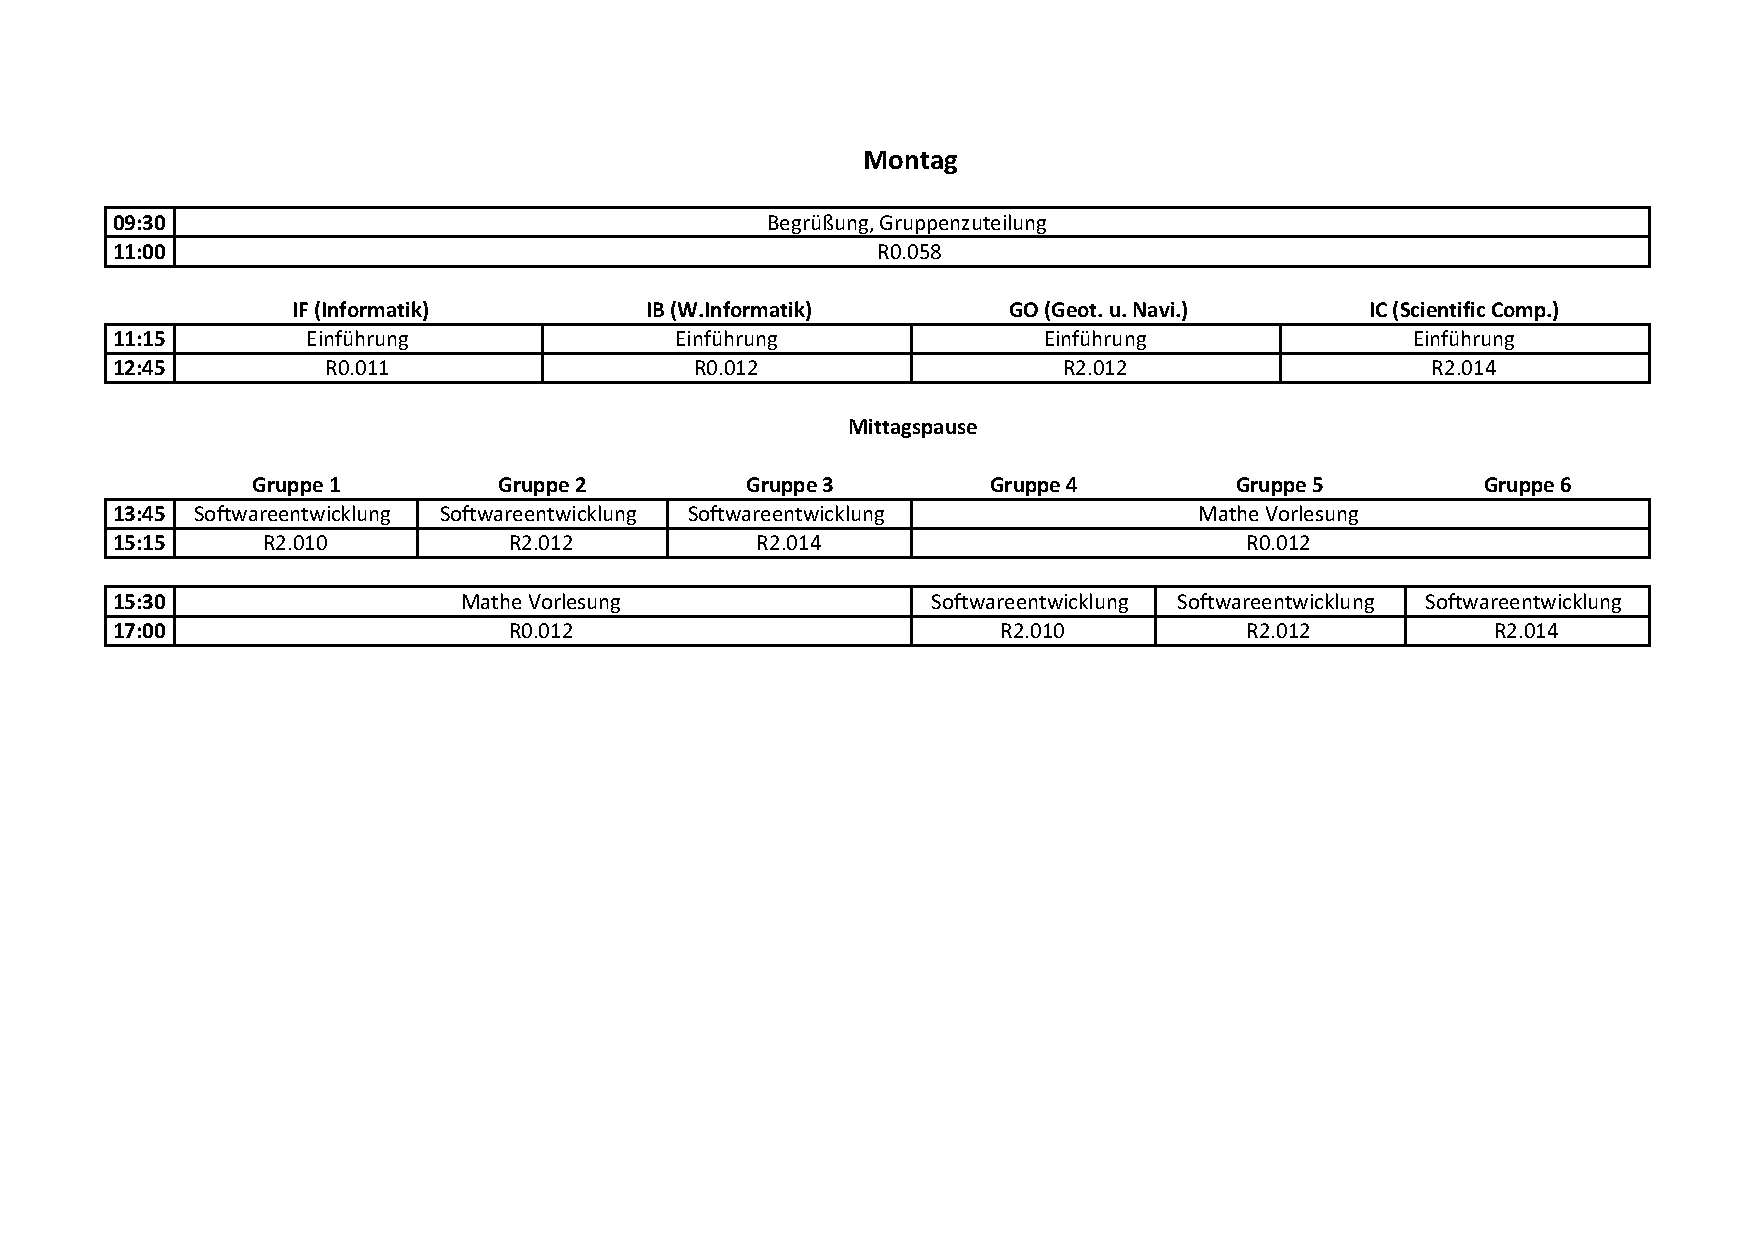
\includepdf[pages=1]{timetable.pdf}
	\includepdf[pages=2]{timetable.pdf}
	\includepdf[pages=3]{timetable.pdf}
	\includepdf[pages=4]{timetable.pdf}
	\includepdf[pages=5]{timetable.pdf}
}

\begin{frame}
\frametitle{Gruppeneinteilung}
\end{frame}

\begin{frame}
\frametitle{Ende}
\begin{center}
Danke für eure Aufmerksamkeit\\
und\\
viel Spaß im Vorkurs!
\end{center}
\end{frame}

\end{document}
